\documentclass{beamer}
\mode<presentation>
\title[SKI: The Computational Search Engine.\hspace{1.6cm}\insertframenumber/\inserttotalframenumber]{SKI: The Semantic Search \& Computational Engine.}
\author[Shashi Kant]{Shashi Kant}
\date{\today \\ \texttt{shashikant@tenhash.com}}
\institute{Department of Computer Science \& Engineering \\ National Institute of Technology, Jamshedpur}

\usepackage{beamerthemesplit}
\usetheme{Frankfurt}
\useoutertheme{default}
\usecolortheme{seahorse}
\logo{sk}



\begin{document}
\begin{frame}
   \titlepage
\end{frame}



\begin{frame}
 \frametitle{Computational cum Semantic Search Engine}
 \framesubtitle{Just another search engine?}
 \begin{block}{Semantic Search?} \pause
 \begin{enumerate}
   \item  Well! what is this \alert{Semantic Search} and how is it different from current search engines? 
   \pause
   \item what current search engines can't answer?
   \pause
   \item How can it be useful?
   \pause
   \item Any existing semantic search engine? 
   \pause
   \item What is computational engine?
  \end{enumerate}
 \pause
 \end{block}
 
 Before diving into answers, we first need to understand the limitations of present search engines.
 
 
\end{frame}

\begin{frame}[t]

 \frametitle{Present search engines can be better}
 \pause
 \begin{itemize}
  \item google search results can be more specific.
  \pause
  \item google or even wikipedia don't give us answer.
 \end{itemize}
\end{frame}
\begin{frame}
   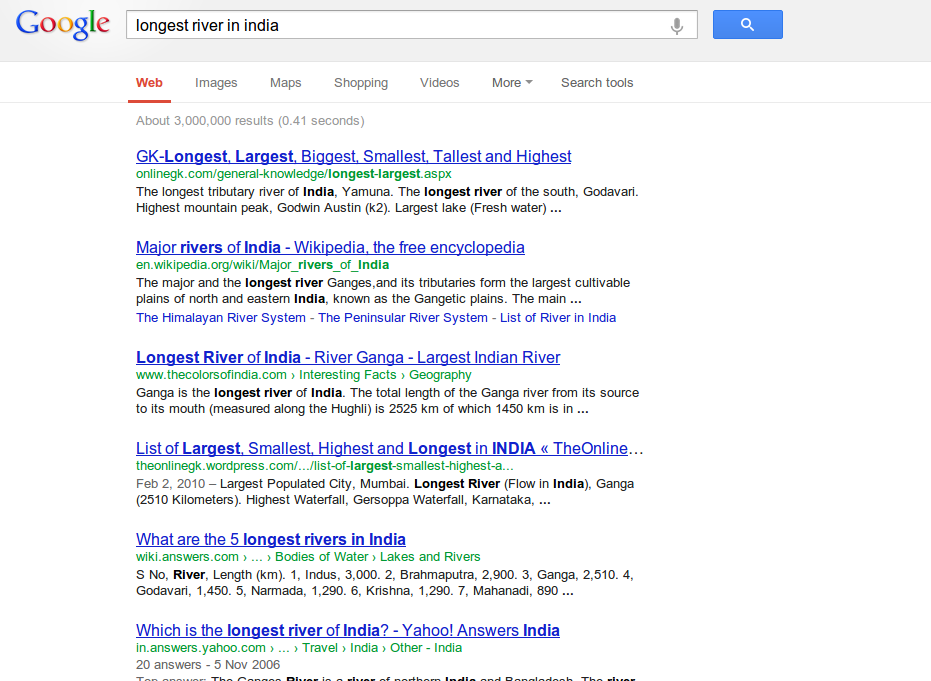
\includegraphics[width=12cm,height=8cm]{two.png}
\end{frame}

\begin{frame}
 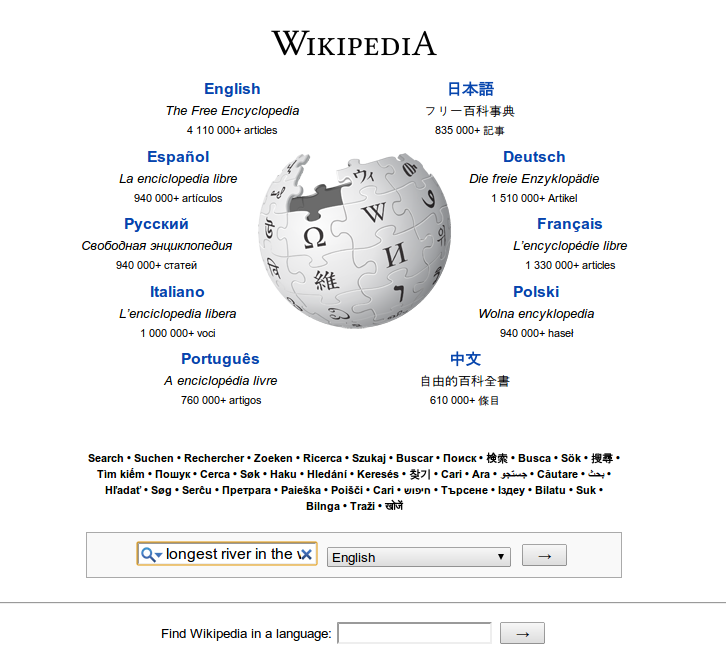
\includegraphics[width=12cm,height=8cm]{four.png}
\end{frame}

\begin{frame}
 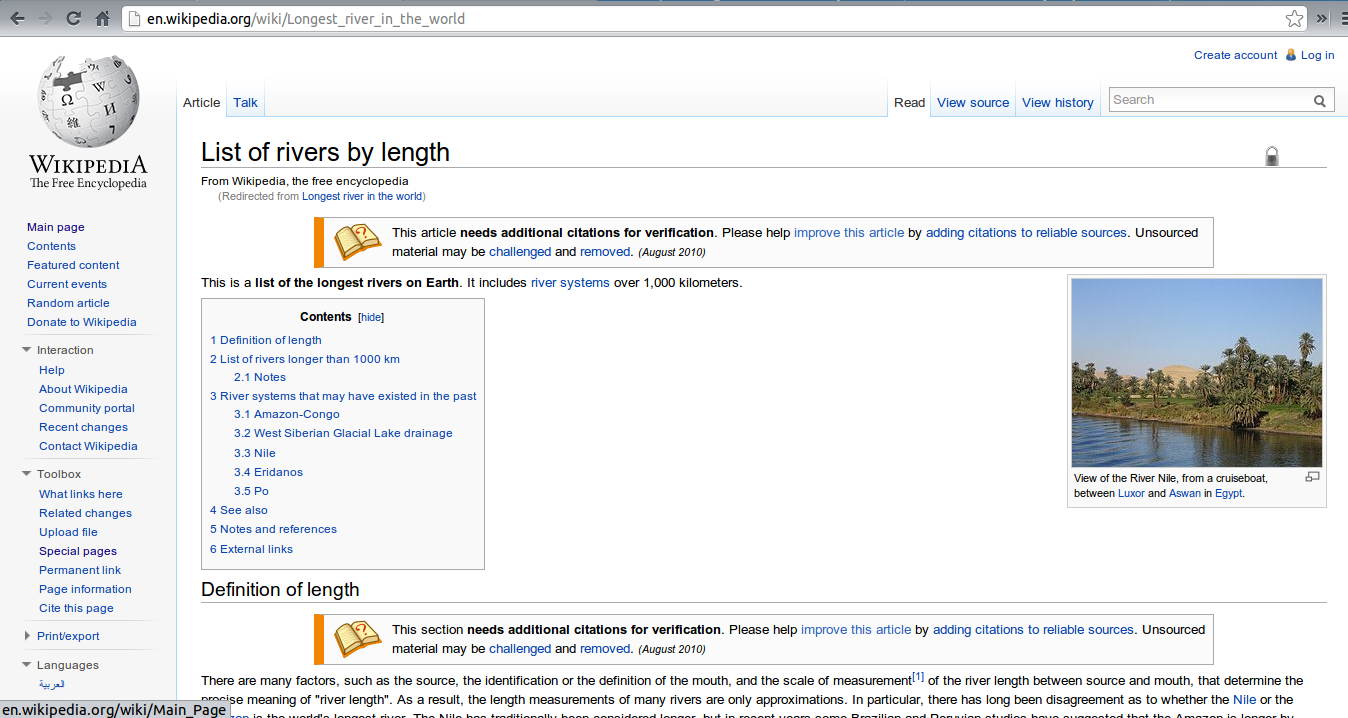
\includegraphics[width=12cm,height=8cm]{three.png}
\end{frame}

\begin{frame}
  \frametitle{Present search engines can be better}
 \begin{itemize}
  \item google search results can be more specific.
    \item google or even wikipedia don't give us answer.
    \pause
  \item sometimes, computational engines can be more useful

 \end{itemize}
\end{frame}

\begin{frame}
 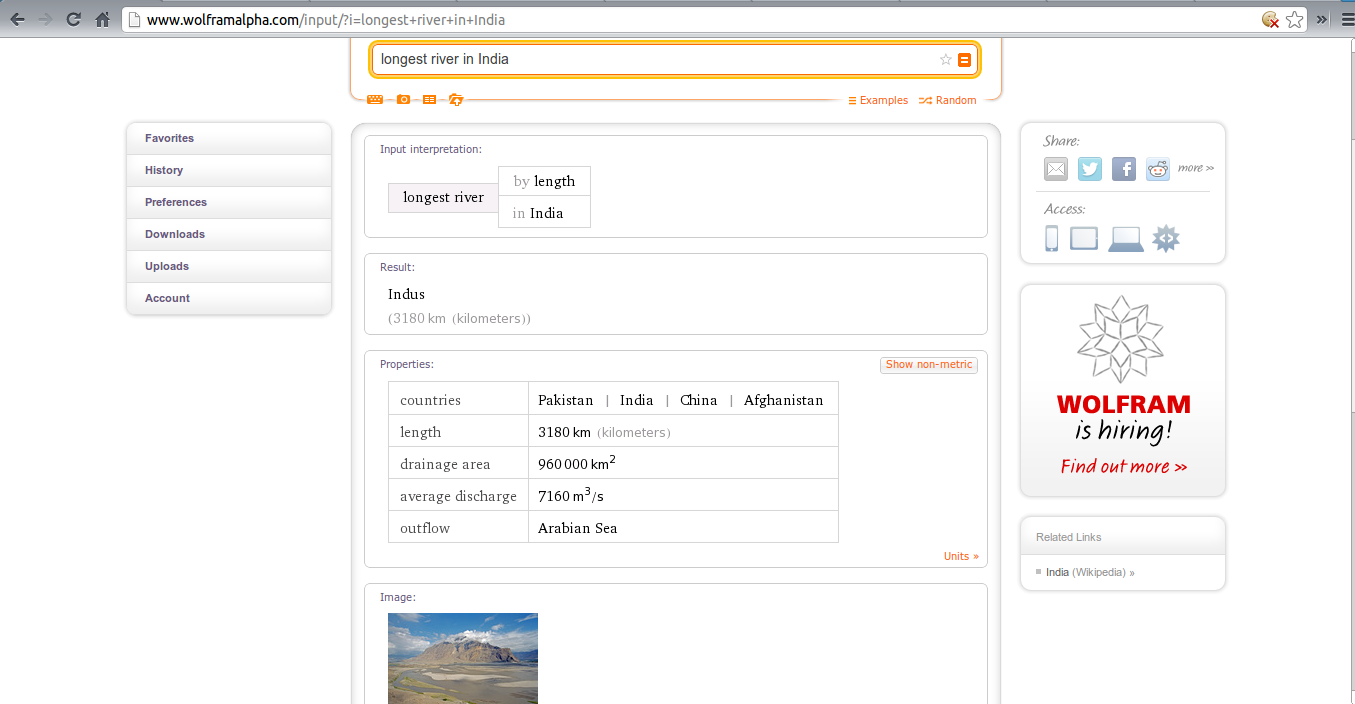
\includegraphics[width=12cm,height=8cm]{one.png}
\end{frame}


\begin{frame}
   \frametitle{Present search engines can be better}
 \begin{itemize}
  \item google search results can be more specific.
   \item google or even wikipedia don't give us answer.
  \item sometimes, computational engines can be more useful
 
  \pause
  \item Facebook's graph search can't deduce relations using given set of rules.
 \end{itemize}
\end{frame}

\begin{frame}
 \frametitle{Features of SKI}
 \begin{block}{It enjoys features of both worlds}
 \begin{enumerate}
  \item Directly give answers to the questions.
  \pause
  \item Produce User specific search results.
  \pause
  \item Can solve complex mathematical problems.
  \pause
  \item Can decuce relations from given set of rules.
 \end{enumerate}
 \end{block}
\end{frame}

\begin{frame}
 \frametitle{Features of SKI}
 \begin{example}
  \begin{itemize}

  \item  \alert{Question:} Can Pypi give birth to new offspring?
   \pause	
   \item \alert{Rules:}
   \item Pypi is a cat.
   \item Cats are mammals.
   \item Mammals can give birth to new offspring.
   \pause
   \item \alert{Answer:} Yes, Pypi can give birth to a new offspring.  
  \end{itemize}
 \end{example}
\end{frame}


\begin{frame}
 \frametitle{Questions}
 \begin{block}{Join me in this project}
  \begin{itemize}
  \pause
  \item You can always reach me at \texttt{shashikant@tenhash.com} and \texttt{http://blog.tenhash.com} 
  \pause
   \item Suggestions
    \pause
   \item Questions
   \pause
   \item \textbf{Thank You !}
  \end{itemize}

 \end{block}

\end{frame}



 

\end{document}
